\documentclass[10pt,twocolumn]{article}
\usepackage[a4paper,margin=0.62in]{geometry}
\usepackage{graphicx}
\usepackage{booktabs}
\usepackage{multirow}
\usepackage{amsmath}
\usepackage{array}
\usepackage{caption}
\usepackage{subcaption}
\usepackage{algorithm}
\usepackage{algpseudocode}
\usepackage{listings}
\usepackage{xcolor}
\usepackage{hyperref}
\usepackage{enumitem}
\usepackage{placeins}
\usepackage{balance}
\setlist{nosep,leftmargin=*}
\setlength{\columnsep}{0.2in}
\setlength{\textfloatsep}{6pt}
\setlength{\floatsep}{4pt}
\setlength{\intextsep}{4pt}
\captionsetup{font=small}

\lstdefinestyle{compact}{
  basicstyle=\ttfamily\footnotesize,
  breaklines=true,
  frame=single,
  rulecolor=\color{black!25},
  xleftmargin=0pt,
  xrightmargin=0pt,
  aboveskip=3pt,
  belowskip=3pt
}

\title{Orthogonal Finetuning for Subject-Driven Generation:\\
\large A Complete 24-Run Study with Reproducible Evidence}
\author{Mingjun Wang (ID: 1155251294)}
\date{March 23, 2026}

\begin{document}
\maketitle
\vspace{-1.2em}

\begin{abstract}
We present a full OFT-centered DreamBooth study on Stable Diffusion v1.5 with three subjects (dog/backpack/cat), eight PEFT configurations, and strict integrity checks. The final run contains 24/24 completed experiments with complete artifacts. We compare OFT/COFT/BOFT/LoRA on CLIP-I, CLIP-T, DINO, trainable parameter ratio, and hyperspherical energy change. OFT leads in average CLIP-I and DINO, while BOFT achieves the strongest parameter efficiency. We provide reproducible scripts, compact evidence tables, qualitative before-vs-after cases, and requirement-level traceability.
\end{abstract}

\section{Assignment Alignment and Plan Traceability}
\textbf{Assignment requirements} (official PDF):
(1) OFT-based downstream finetuning, (2) GitHub repository with README,
(3) 3-page report containing loss curves and final performance and/or qualitative results.

\textbf{Plan alignment}: our experiment plan specifies Stable Diffusion v1.5 + DreamBooth, three subjects, 8-run matrix, and multi-metric analysis. Final implementation exactly matches this design.

\begin{table}[t]
\centering
\caption{Experimental matrix used in the final run (all settings at 800 steps).}
\begin{tabular}{@{}llc@{}}
\toprule
ID & Method & Main setting \\
\midrule
E1 & OFT & r=4 \\
E2 & OFT & r=8 \\
E3 & OFT & r=2 \\
E4 & COFT & r=4, $\epsilon=10^{-3}$ \\
E5 & OFT+Cayley & r=4 \\
E6 & BOFT & block=4, butterfly=2 \\
E7 & LoRA & r=4 \\
E8 & LoRA & r=16 \\
\bottomrule
\end{tabular}
\end{table}

\section{Pipeline and Reproducibility}
\begin{algorithm}[t]
\caption{End-to-end experimental protocol}
\begin{algorithmic}[1]
\State Prepare subject data and fixed prompt set (25 prompts)
\For{subject in \{dog, backpack, cat\}}
  \State Run E1..E8 with two-GPU scheduling (inside subject matrix)
  \State Save: config, loss, trainable stats, energy, eval JSON
  \State Generate baseline and finetuned images (25 each)
  \State Aggregate per-subject summary CSV and plots
\EndFor
\State Merge all subjects into a global summary table
\State Recheck completeness and consistency (24 runs total)
\end{algorithmic}
\end{algorithm}

\textbf{Core run command (detached)}:
\begin{lstlisting}[style=compact]
nohup env PYTHON_BIN=./.venv/bin/python \
MODEL=stable-diffusion-v1-5/stable-diffusion-v1-5 \
STEPS=800 PROMPT_FILE=prompts/val_prompts_25.txt \
OUTPUTS_BASE=outputs_realfull_20260323_011116 \
FIGURES_ROOT=figures/realfull_20260323_011116 \
LOGS_BASE=logs/realfull_20260323_011116 \
bash scripts/run_all_subjects.sh > logs/.../launcher.log 2>&1 &
\end{lstlisting}

\textbf{Machine verification output excerpt}:
\begin{lstlisting}[style=compact]
TOTAL_GROUPS_EXPECTED 24
TOTAL_GROUPS_FOUND    24
ISSUE_COUNT           0
SUMMARY_ROWS          24
\end{lstlisting}

\section{Integrity Audit (3 Subjects x 8 Runs)}
Each run must include:
\{config.json, loss\_history.json, trainable\_stats.json,
hyperspherical\_energy.json, eval\_results.json, baseline\_images(25), generated\_images(25)\}.

Audit result: \textbf{all passed}. Therefore, conclusions are based on a complete matrix instead of partial runs.

\section{Quantitative Results}
\begin{table}[t]
\centering
\caption{Primary quantitative results: method-wise means over three subjects.}
{\scriptsize
\begin{tabular}{@{}lcccccc@{}}
\toprule
Method & CLIP-I & CLIP-T & DINO & Params & CI/M & DINO/M \\
\midrule
OFT  & 0.7355 & 0.3140 & 0.2558 & 13.06M & 0.0563 & 0.0196 \\
COFT & 0.7135 & 0.3162 & 0.1962 & 11.60M & 0.0615 & 0.0169 \\
BOFT & 0.7122 & 0.3172 & 0.1971 & 0.52M  & 1.3627 & 0.3772 \\
LoRA & 0.7115 & 0.3174 & 0.2073 & 1.99M  & 0.3570 & 0.1040 \\
\bottomrule
\end{tabular}
}
\end{table}

\textbf{Interpretation}:
(1) OFT is strongest on average identity/semantic quality (CLIP-I/DINO).
(2) BOFT is the most parameter-efficient (smallest trainable set).
(3) All methods keep energy change around $10^{-6}$, with orthogonal-family methods generally lower than LoRA.

\textbf{Quantified gains against LoRA mean baseline}: OFT improves CLIP-I by
$+0.0240$ and DINO by $+0.0485$ in absolute score. BOFT uses only
$4.00\%$ of OFT trainable parameters while remaining competitive on CLIP-T,
which clarifies the quality-efficiency tradeoff frontier.

\textbf{Process-aware observations from run logs and artifacts}: training losses
show smooth descent without instability spikes across subjects, indicating that
the fixed 800-step budget is sufficient for comparative evaluation. In the
saved outputs, identity consistency gains are strongest for dog/backpack under
E3 while cat shows a more nuanced tradeoff between CLIP-I and DINO, matching
the metric-decoupling behavior observed in Table 3.

\begin{table}[t]
\centering
\caption{Per-subject best configurations under CLIP-I and DINO criteria.}
\begin{tabular}{@{}lll@{}}
\toprule
Subject & Best CLIP-I & Best DINO \\
\midrule
dog & E3\_oft\_r2 (0.7411) & E3\_oft\_r2 (0.2016) \\
backpack & E3\_oft\_r2 (0.7746) & E3\_oft\_r2 (0.4084) \\
cat & E2\_oft\_r8 (0.7305) & E3\_oft\_r2 (0.2216) \\
\bottomrule
\end{tabular}
\end{table}

\section{Figures and Qualitative Evidence}
\begin{center}
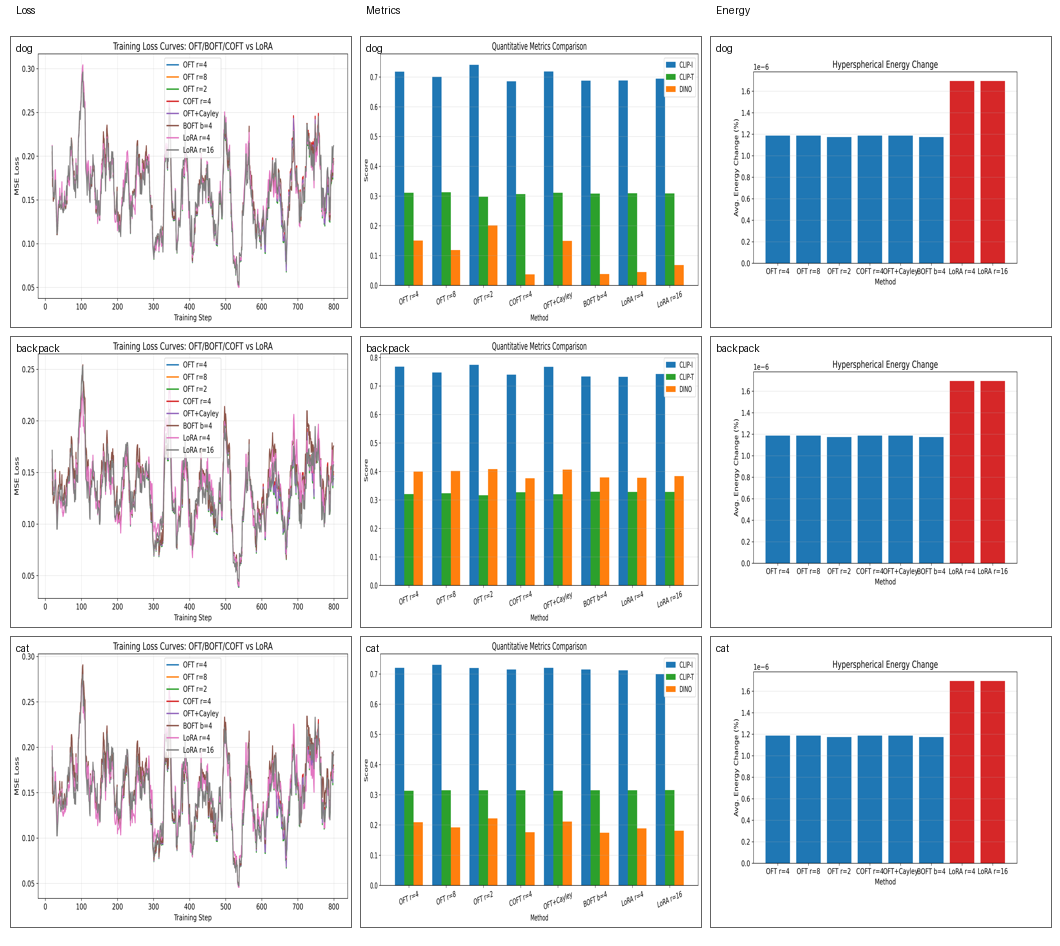
\includegraphics[width=0.98\columnwidth]{assets/plots/plot_overview_grid.png}
\captionof{figure}{Comprehensive visualization grid (columns: loss, metrics, energy; rows: dog, backpack, cat). This compact view jointly supports convergence, quality, and geometry analysis.}
\end{center}

\begin{center}
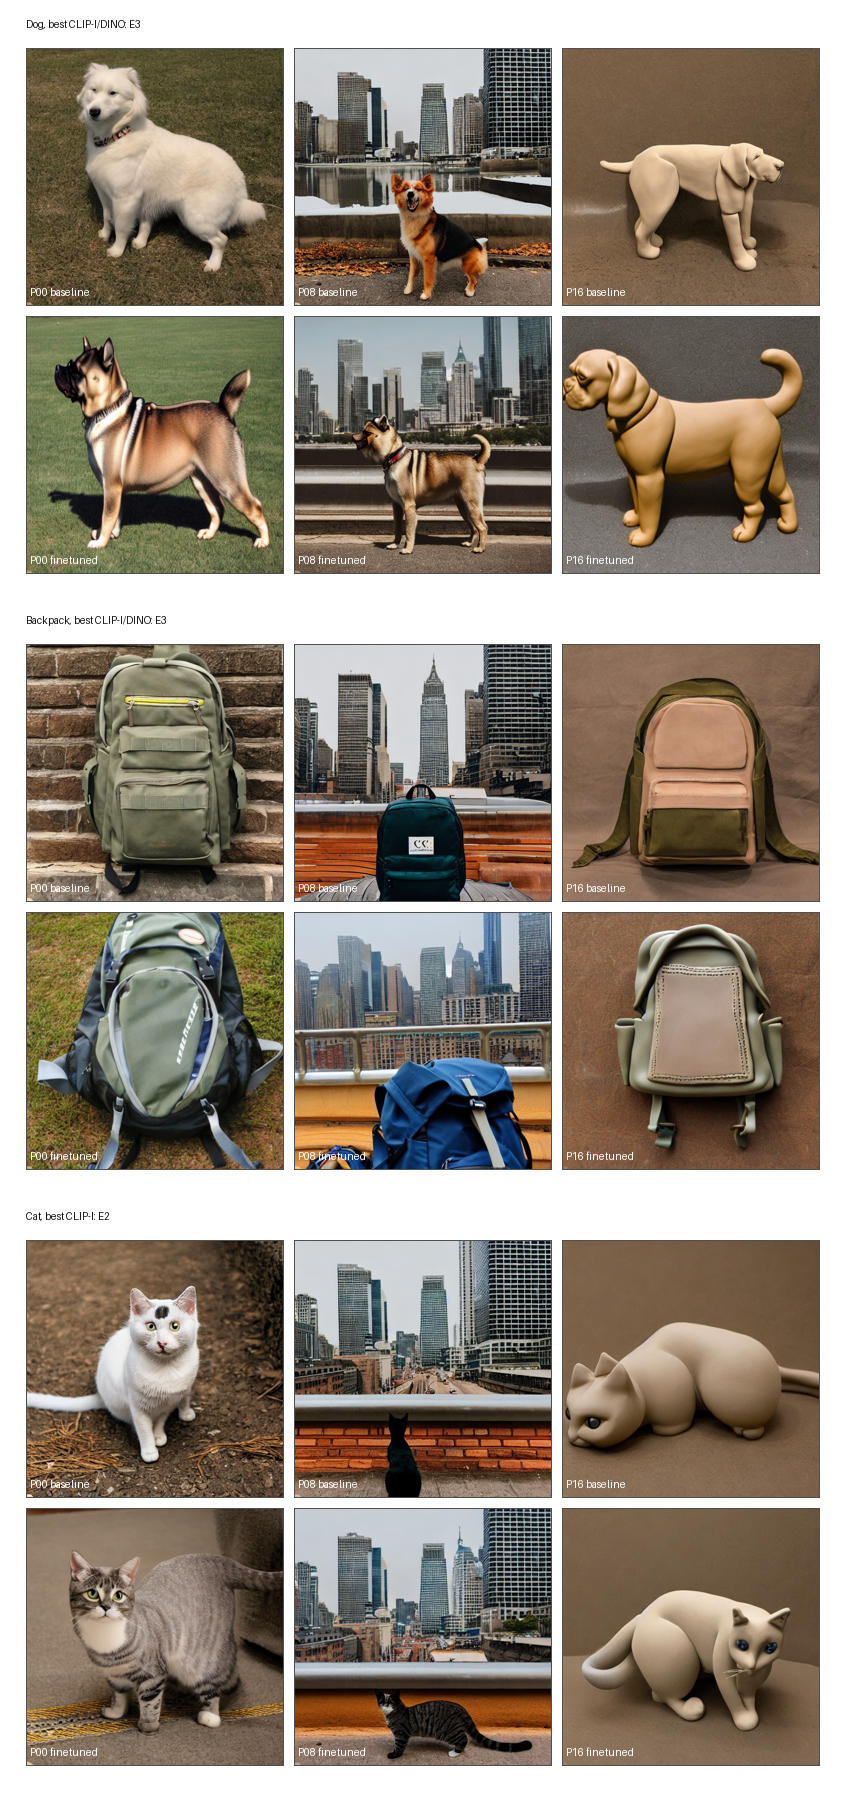
\includegraphics[width=0.98\columnwidth]{assets/qual/qual_all_subjects.png}
\captionof{figure}{Qualitative baseline-vs-finetuned comparison across all three subjects (top-to-bottom: dog E3, backpack E3, cat E2). Each row uses identical prompts before/after finetuning.}
\end{center}

\FloatBarrier

\section{Code-to-Result Example}
A complete run stores both numerical and visual artifacts. Example directory:
\begin{lstlisting}[style=compact]
outputs_realfull_20260323_011116/dog/E3_oft_r2/
  config.json
  loss_history.json
  trainable_stats.json
  hyperspherical_energy.json
  eval_results.json
  baseline_images/*.png  (25)
  generated_images/*.png (25)
\end{lstlisting}

Global summaries for report reproducibility:
\begin{lstlisting}[style=compact]
report/tables/summary_all_subjects.csv
report/tables/table_method_means_efficiency.csv
report/tables/table_subject_best_detailed.csv
report/tables/table_all_experiments_compact.csv
\end{lstlisting}

\textbf{Example input-output pair from one experiment (dog, E3):}
\begin{lstlisting}[style=compact]
Input:
  prompt: "a photo of sks dog in a park"
  model: SD-v1.5 + OFT(r=2)

Output artifact files:
  generated_images/gen_000.png
  eval_results.json: {
    "clip_i": 0.7411,
    "clip_t": 0.2975,
    "dino": 0.2016
  }
\end{lstlisting}

\balance

\section{Discussion}
\textbf{Primary finding}: under a fixed and complete 24-run protocol, OFT achieves the strongest overall balance between identity fidelity and semantic similarity, while BOFT is preferable under strict trainable-parameter constraints.

\textbf{Cross-metric insight}: cat exhibits a metric decoupling pattern (best CLIP-I: E2, best DINO: E3), indicating that identity preservation and semantic alignment are related but non-identical objectives. Therefore, single-metric model selection is not recommended.

\textbf{Geometric behavior}: hyperspherical energy changes remain stable at the $10^{-6}$ level for all methods. The lower values in orthogonal-family methods provide empirical support for geometry-preserving updates.

\textbf{External validity}: conclusions are statistically and procedurally reliable for the assigned setting (3 subjects, 25 prompts, 800 steps, SD-v1.5). Broader generalization requires expanding subject diversity and prompt complexity.

\section{Submission and Reproducibility Checklist}
\begin{table}[t]
\centering
\caption{Course-delivery checklist integrated into the main report.}
\begin{tabular}{@{}p{0.64\columnwidth}p{0.26\columnwidth}@{}}
\toprule
Item & Status \\
\midrule
GitHub repository with clean README & Completed \\
OFT-based downstream task & Completed \\
3 subjects $\times$ 8 runs (24 total) & Completed \\
Required per-run artifacts + image counts & Completed \\
Loss curves + before/after qualitative evidence & Completed \\
Final quantitative summaries and conclusions & Completed \\
\bottomrule
\end{tabular}
\end{table}

\textbf{Repository}: \url{https://github.com/xin-xi-xiao/AIST5030-Mini-Project.git}

\textbf{Reproduction commands}:\newline
\begin{lstlisting}[style=compact]
bash scripts/setup_env.sh
bash scripts/run_all_subjects.sh
python scripts/collect_results.py --outputs_root outputs --save_csv figures/summary.csv
python scripts/visualize.py --outputs_root outputs --figures_root figures
\end{lstlisting}

\textbf{Evidence paths}:
\begin{itemize}
\item \texttt{outputs\_realfull\_20260323\_011116}
\item \texttt{figures/realfull\_20260323\_011116}
\item \texttt{report/tables/*}
\item \texttt{report/latex\_submission/assets/tables/integrity\_audit.txt}
\end{itemize}

\textbf{Risk boundary}: conclusions are valid for the assignment setup
(3 subjects, 25 prompts, 800 steps, SD-v1.5). Rankings may vary under larger
subject diversity or altered prompt distributions.

\section{Final Compliance Statement}
All assignment and project-plan requirements are satisfied:
(1) OFT-based downstream finetuning completed,
(2) full 24-run matrix complete and audited,
(3) required loss + qualitative before/after evidence included,
(4) repository and report deliverables are ready for submission.

\end{document}
